\section{Studio di fattibilità delle possibili soluzioni}
Per poter comprendere le soluzioni di seguito proposte è necessario conoscere il software \glossario{OSS}, presentato alla Sezione \ref{oss}.
La seguente immagine presenta il funzionamento del nuovo sistema PadovaCard nel suo complesso.
Per maggiori dettagli vedere l'analisi dei requisiti alla Sezione \ref{analisideirequisiti}.
\begin{figure}[H]
\centering
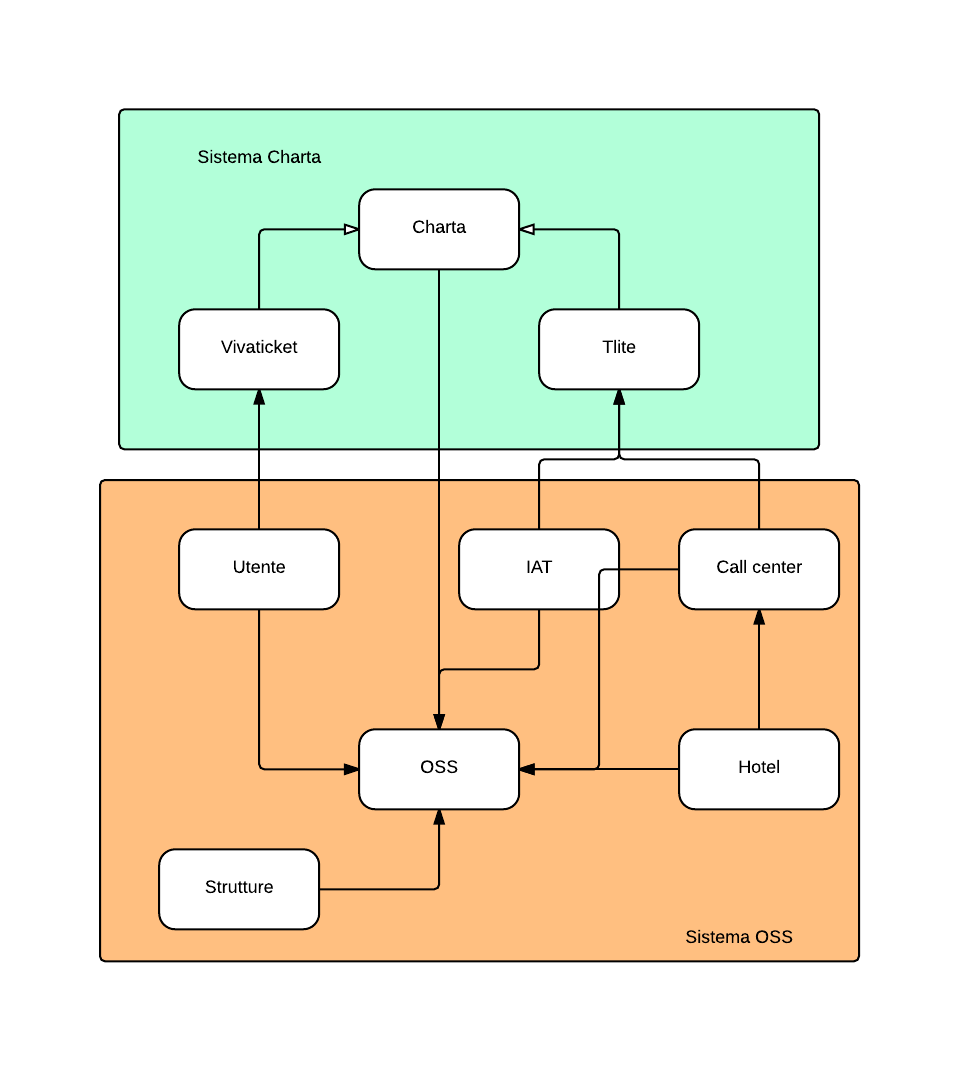
\includegraphics[width=0.9\textwidth]{images/Schema_introduttivo.png}
\caption{Architettura di alto livello di OSS}
\end{figure}

\subsection{Espansione del sistema OSS}
Per questa soluzione non è prevista la produzione di un sistema ex-novo, ma un ampliamento del sistema \glossario{OSS} già esistente affinchè soddisfi i requisiti richiesti.
\begin{figure}[H]
\centering
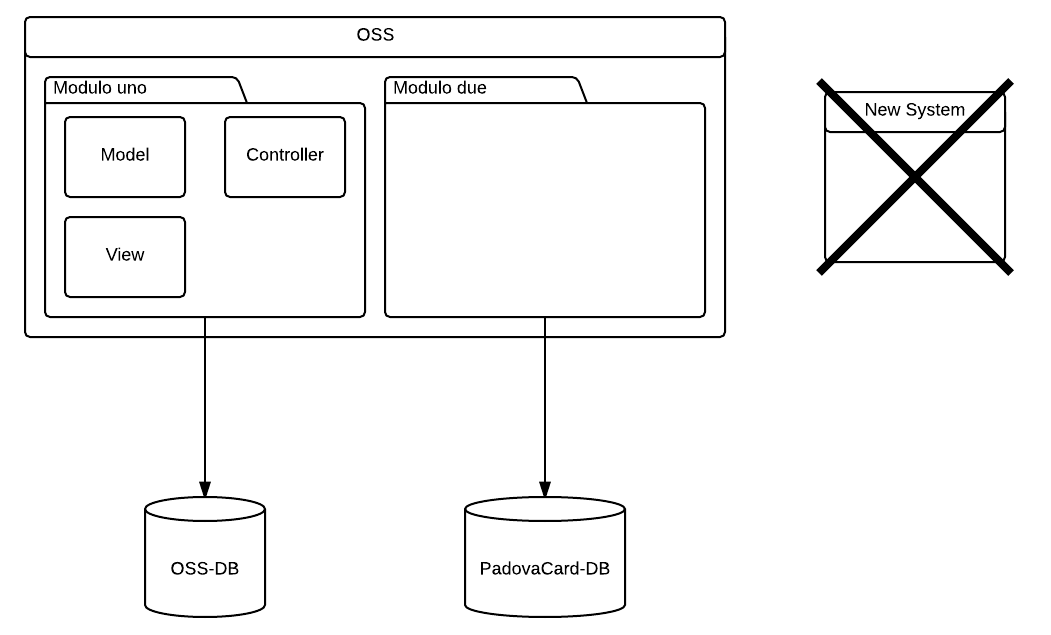
\includegraphics[width=0.7\textwidth]{images/Espansione_del_sistema_OSS.png}
\caption{Diagramma della soluzione: Espansione del sistema OSS}
\end{figure}
Nella figura tutti i componenti interni al modulo uno sono quelli già esistenti che non andranno modificati.
I componenti all'interno del modulo due sono quelli che verranno progettati e sviluppati per soddisfare i requisiti annessi alla nuova PadovaCard.\\

Il database \glossario{OSS} è quello già presente mentre il database PadovaCard è quello che andrà creato. In alternativa si può utilizzare un unico database e creare nuove tabelle per la gestione della PadovaCard.
Questa soluzione soddisfa il requisito di avere un unica piattaforma per gestire tutto, dalla vendita della PadovaCard, alla vendita di altri articoli, alla gestione dei pagamenti e degli operatori.\\

Uno svantaggio è che il tirocinante, se pur a conoscenza del linguaggio PHP e dell'architettura MVC, non ha mai sviluppato con CakePHP, inoltre dovrebbe studiare il funzionamento del sistema esistente nel dettaglio. Tale studio può limitarsi alle sezioni del software di interesse, ma si prevede un costo di apprendimento iniziale elevato.\\
\textbf{Vantaggi:}
\begin{itemize}
\item Non viene creato un nuovo sistema;
\item Necessaria meno documentazione;
\item Il pagamento di PadovaCard e altri articoli è unico;
\item I dati relativi alla PadovaCard sono logicamente separati, mentre quelli amministrativi sono accorpati.
\end{itemize}
\textbf{Svantaggi:}
\begin{itemize}
\item Necessario l'apprendimento del funzionamento di OSS;
\item Necessario l'apprendimento del funzionamento di CakePHP;
\item Rischio di introdurre errori in un sistema funzionante;
\end{itemize}

\subsection{Nuovo sistema per gli acquisti}
In questa soluzione si prevede di progettare e realizzare un nuovo sistema che si occuperà della vendita delle PadovaCard e degli altri articoli. Il sistema OSS resterà presente in parallelo per la gestione delle rimanenti necessità.

\begin{figure}[H]
\centering
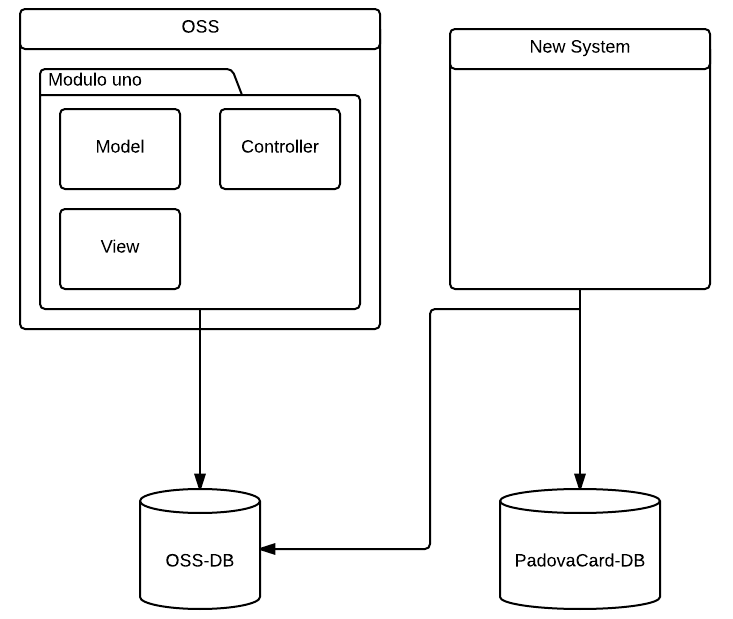
\includegraphics[width=0.7\textwidth]{images/Nuovo_sistema_per_gli_acquisti.png}
\caption{Diagramma della soluzione: Nuovo sistema per gli acquisti}
\end{figure}
A differenza della soluzione precedente in questo caso il sistema OSS ora esistente non viene modificato, e si crea un nuovo sistema, identificato in figura come come new System. Tale sistema non interagisce in alcun modo con il sistema OSS, ma comunica invece con il database OSS per la scrittura degli acquisti, mentre comunicherà con il database PadovaCard per tutti i dettagli riguardanti le sole PadovaCard.\\

Tale soluzione presenta il vantaggio per il tirocinante di non dover apprendere CakePHP e il funzionamento di OSS, ma c'è il rischio di una frammentazione dei dati. \\
\textbf{Vantaggi:}
\begin{itemize}
\item Nuovo sistema, separato ed indipendente per la vendita della PadovaCard;
\item Il sistema OSS non viene modificato;
\item Il pagamento di PadovaCard e altri articoli è unico;
\item I dati relativi alla PadovaCard sono logicamente separati, mentre quelli amministrativi sono accorpati.
\end{itemize}
\textbf{Svantaggi:}
\begin{itemize}
\item Necessaria la progettazione di un nuovo sistema;
\item Il codice sorgente relativo a vendita e pagamento verrebbe duplicato;
\item Necessaria una maggiore documentazione;
\item Si hanno due sistemi che in parte fanno la stessa cosa.
\end{itemize}

\subsection{Sistema ibrido}
Si tratta di una soluzione che ibrida le due appena viste. In questo caso viene creato un nuovo sistema, che si occuperà della sola vendita della PadovaCard (ed eventualmente dei singoli accessi ai luoghi d'interesse), mentre OSS continuerà a vendere tutti gli altri articoli. 
I due sistemi comunicheranno tra loro e l'operatore potrà passare da uno all'altro in modo automatico in base a cosa desidera vendere. \\

Il pagamento finale sarà possibile su entrambe le piattaforme e comprenderà gli articoli venduti su entrambe.

\begin{figure}[H]
\centering
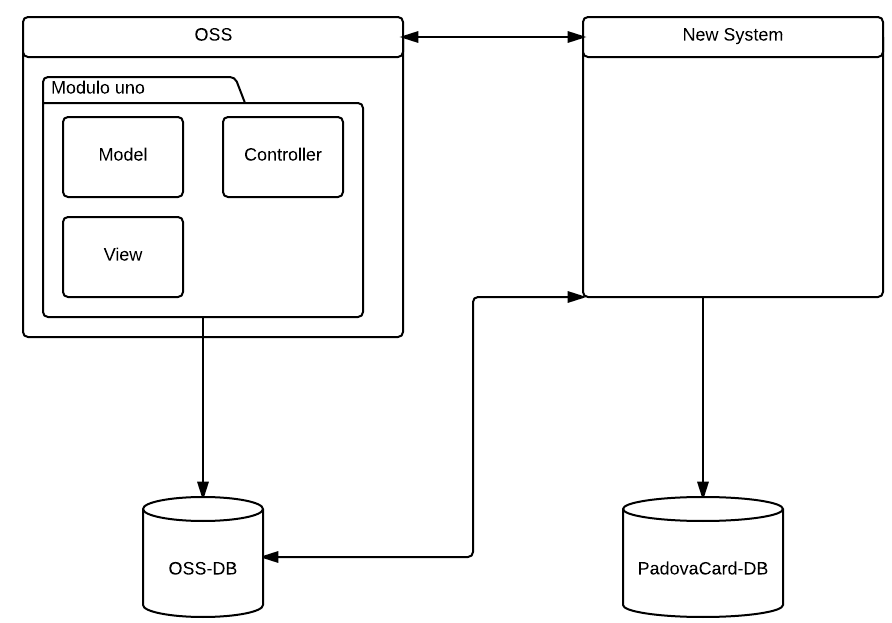
\includegraphics[width=0.7\textwidth]{images/Sistema_ibrido.png}
\caption{Diagramma della soluzione: Sistema ibrido}
\end{figure}
Questa soluzione prevede che il sistema OSS non venga modificato se non per il redirect al nuovo sistema e la conferma al nuovo sistema dell'avvenuto pagamento. 
Nel database OSS saranno salvati i record di vendita, comprese le PadovaCard, ma tutti i dettagli relativi ad esse saranno separati nel database PadovaCard (o in un'altra tabella nello stesso database). \\
\textbf{Vantaggi:}
\begin{itemize}
\item Nuovo sistema, separato ed indipendente per la vendita della PadovaCard;
\item Il sistema OSS viene modificato solo in superficie, con un costo basso;
\item Per l'operatore il pagamento di PadovaCard e altri articoli è unico;
\item I dati relativi alla PadovaCard sono logicamente separati, mentre quelli amministrativi sono accorpati.
\end{itemize}
\textbf{Svantaggi:}
\begin{itemize}
\item Necessaria la progettazione di un nuovo sistema;
\item L'operatore passando da un sistema all'altro si troverebbe una diversa interfaccia;
\item Necessaria una maggiore documentazione;
\end{itemize}

\subsection{Conclusioni}
La soluzione due, Nuovo sistema per gli acquisti, presenta maggiori svantaggi rispetto ai vantaggi, e per questo è stata immediatamente scartata. \\

Le soluzioni uno e tre hanno molti vantaggi in comune, come la separazione logica dei dati relativi alla PadovaCard e l'unificazione del sistema di pagamento, ma ritengo che la soluzione uno presenti un minor costo di sviluppo in termini di uomo/ora, e sia quindi da preferire.